\documentclass[12pt]{article}
\usepackage{fullpage}
\usepackage{graphicx}
\usepackage{hyperref}
\usepackage{bm}
\usepackage{amsmath}
\usepackage{amssymb}
\usepackage{derivative}
\usepackage{bm}
\usepackage{comment}
\usepackage{cancel}
\usepackage{xcolor}
\usepackage{float}

\begin{document}
\title{General Relativity: Homework 5}
\author{Koichiro Takahashi}
\maketitle

\section*{Problem.1}
$K^{\mu}$ is a Killing vector if
\begin{align}
\nabla_{\nu} K_{\mu} + \nabla_{\mu} K_{\nu} = 0
\end{align}
Assume $\partial_0 g_{\mu \nu} = 0$. In this case, we can show a constant vector $K^{\mu} = \left(1, 0, 0, 0\right)$ is a Killing vector by using a formula
\begin{align}
\nabla_{\nu} K_{\mu} = \partial_{\nu} K_{\mu} - \Gamma^{\alpha}_{\nu \mu} K_{\alpha}
\end{align}
Here, 
\begin{align}
K_{\mu} = g_{\mu \nu} K^{\nu} = g_{\mu 0}
\end{align}
so that
\begin{align}
\nabla_{\nu} K_{\mu} + \nabla_{\mu} K_{\nu} &= \partial_{\nu} K_{\mu} - \Gamma^{\alpha}_{\nu \mu} K_{\alpha} + \partial_{\mu} K_{\nu} - \Gamma^{\alpha}_{\mu \nu} K_{\alpha}\\
&= \partial_{\nu} g_{\mu 0} - \Gamma^{\alpha}_{\nu \mu} g_{\alpha 0} + \partial_{\mu} g_{\nu 0} - \Gamma^{\alpha}_{\mu \nu} g_{\alpha 0} \\
&= \partial_{\nu} g_{\mu 0} + \partial_{\mu} g_{\nu 0} - 2 \Gamma^{\alpha}_{\nu \mu} g_{\alpha 0} ~~\left(\because \Gamma^{\alpha}_{\mu \nu} = \Gamma^{\alpha}_{\nu \mu} \right)\\
&= \partial_{\nu} g_{\mu 0} + \partial_{\mu} g_{\nu 0} - g_{\alpha 0} g^{\alpha \sigma} \left( \partial_{\mu} g_{\nu \sigma} + \partial_{\nu} g_{\mu \sigma} - \partial_{\sigma} g_{\mu \nu} \right)
\end{align}
Here, 
\begin{align}
g_{\alpha 0} g^{\alpha \sigma} = g_{0 \alpha} g^{\alpha \sigma}  = \delta_{0}^{~\sigma}
\end{align}
Thus,
\begin{align}
\nabla_{\nu} K_{\mu} + \nabla_{\mu} K_{\nu} &= \partial_{\nu} g_{\mu 0} + \partial_{\mu} g_{\nu 0} - \delta_{0}^{~\sigma} \left( \partial_{\mu} g_{\nu \sigma} + \partial_{\nu} g_{\mu \sigma} - \partial_{\sigma} g_{\mu \nu} \right)\\
&= \partial_{\nu} g_{\mu 0} + \partial_{\mu} g_{\nu 0} - \left( \partial_{\mu} g_{\nu 0} + \partial_{\nu} g_{\mu 0} - \partial_{0} g_{\mu \nu} \right)\\
&= \partial_{0} g_{\mu \nu} = 0 ~~\left(\because \mathrm{Assumption} \right)
\end{align}
\section*{Problem.2}
When $G =M =c = 1$, the Schwarzschild metric give the line element
\begin{align}
ds^2 = - \left(1 - \frac{2}{r}\right) dt^2 +\left(1 - \frac{2}{r}\right)^{-1} dr^2 + r^2 d \theta^{2} + r^2 \sin^{2}{\theta} d \phi^{2}
\end{align}
(i)Assume $p_{t} = - \omega_{\infty}$. At far away from the black hole, $g_{\mu \nu} = \eta_{\mu \nu}$, so that
\begin{align}
E = p_{t} = \eta_{t t} p^{t} = - \omega_{\infty} \Leftrightarrow p^{t} = \omega_{\infty}
\end{align}
Therefore, the 4-momentum
\begin{align}
p^{\mu} = \frac{d x^{\mu}}{d \lambda} = \left( \omega_{\infty}, \omega_{\infty}, 0, 0 \right)
\end{align}
since $x = t, y = b = const., z = 0$.\\
(ii)
The transformation matrix is given by
\begin{align}
\frac{\partial x^{\mu'}}{\partial x^{\mu}} =
\begin{pmatrix}
 1 & 0 & 0 & 0 \\
 0 & \sin{\theta} \cos{\phi} & \cos{\theta} \cos{\phi}/ r & - \sin{\phi}/\left(r \sin{\theta}\right) \\
 0 & \sin{\theta} \sin{\phi} & \cos{\theta} \sin{\phi}/r & \cos{\phi}/\left(r \sin{\theta}\right) \\
 0 & \cos{\theta} & - \sin{\theta}/r & 0 \\
\end{pmatrix}
\end{align}
where the primed coordinates are the spherical coordinates and the umprimed coordinates are the Cartesian coordinates.\\
Therefore, the 4-momentum transformation
\begin{align}
p^{\mu'} &= p^{\mu} \frac{\partial x^{\mu'}}{\partial x^{\mu}}\\
&=
\left( \omega_{\infty}, \omega_{\infty}, 0, 0 \right)
\begin{pmatrix}
 1 & 0 & 0 & 0 \\
 0 & \sin{\theta} \cos{\phi} & \cos{\theta} \cos{\phi}/ r & - \sin{\phi}/\left(r \sin{\theta}\right) \\
 0 & \sin{\theta} \sin{\phi} & \cos{\theta} \sin{\phi}/r & \cos{\phi}/\left(r \sin{\theta}\right) \\
 0 & \cos{\theta} & - \sin{\theta}/r & 0 \\
\end{pmatrix}
\\
&= \left( \omega_{\infty}, \omega_{\infty} \sin{\theta} \cos{\phi}, \omega_{\infty} \cos{\theta} \cos{\phi}/ r, - \omega_{\infty} \sin{\phi}/\left(r \sin{\theta}\right) \right)
\end{align}
Especially at $y = b, z = 0$, i.e. $\sin{\phi} = b / r, \theta = \pi/2$,
\begin{align}
p^{\mu'} = \left( \omega_{\infty}, \omega_{\infty} \cos{\phi}, 0, - b\,\omega_{\infty}/r^2 \right)
\end{align}
Thus, 
\begin{align}
p_{\phi} = \eta_{\phi \phi} p^{\phi} = - b\,\omega_{\infty}
\end{align}
(iii) The Schwarzschild metric at $\theta = \pi/2$ is given by
\begin{align}
g_{\mu' \nu'} = \mathrm{diag} \left(- \left(1 - \frac{2}{r}\right), \left(1 - \frac{2}{r}\right)^{-1}, r^2, r^2 \right)
\end{align}
In this case, $p_{\phi}$ anywhere along the trajectory of the photon is constant since $\partial_{\phi} g_{\mu' \nu'} = 0$. As a consequence, one can define a Killing vector $K^{\mu'} = \left(0, 0, 0, 1\right)$, which satisfies
\begin{align}
\nabla_{\nu'} K_{\mu'} + \nabla_{\mu'} K_{\nu'} = 0
\end{align}
so that $p_{\phi} = K_{\phi} p^{\phi} = - b\,\omega_{\infty} = const.$\\
By the same discussion, the metric is time-independent, and from the result of the Problem.1, $p_{t} = \omega_{\infty} = const.$\\
(iv)
\begin{figure}[H]
  \begin{center}
  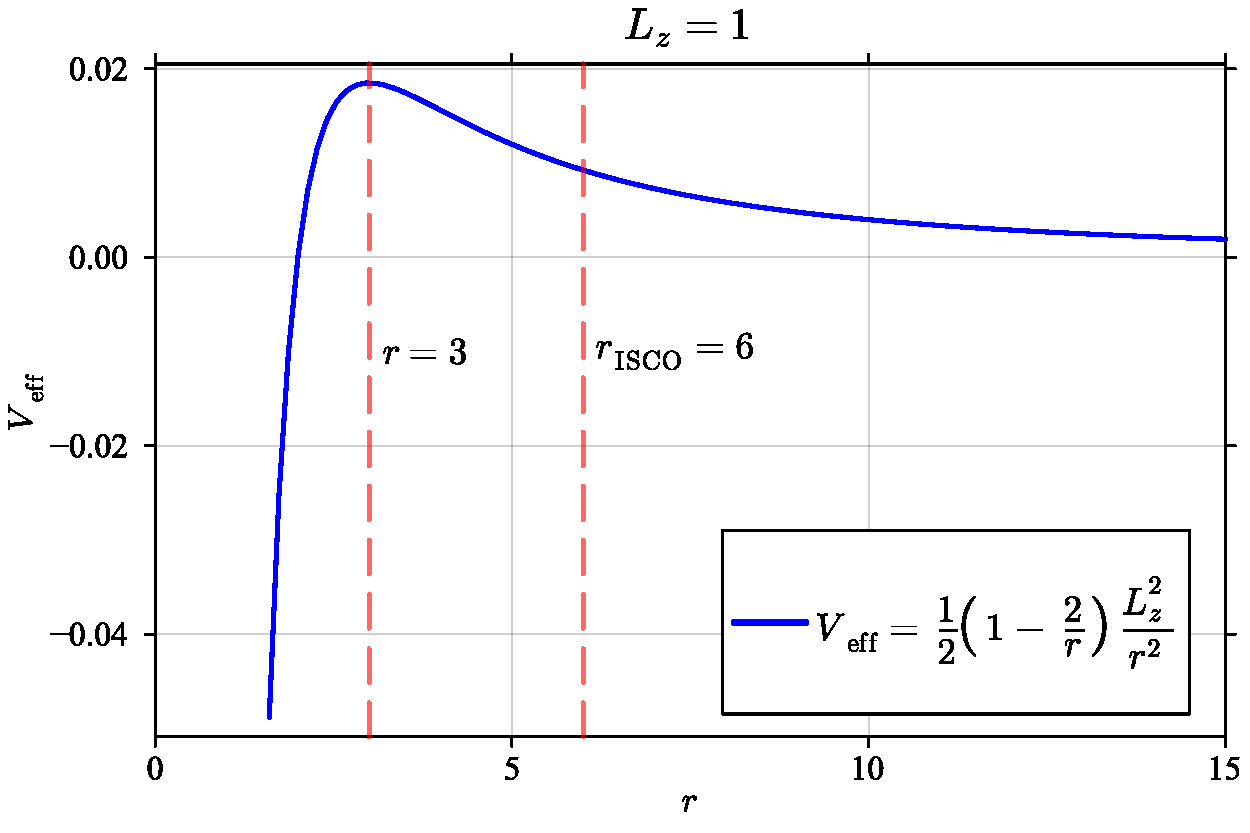
\includegraphics[width=0.7\linewidth]{Massless_Effective_potential.pdf}
  \caption{The effective potential of massless particles in the Schwarzschild metric.}
  \label{Curves}
  \end{center}
\end{figure}
(v)
The effective potential of massless particles in the Schwarzschild metric is given by
\begin{align}
V_{\mathrm{eff}}^{m =0} = \frac{1}{2}\left(1 - \frac{2}{r}\right) \frac{L_z^2}{r^2}
\end{align}
Since the energy is conserved, the maximum of the potential is the closest point to the black hole that can reach and still escape to infinity.
By taking its derivative,
\begin{align}
\frac{\partial}{\partial r} V_{\mathrm{eff}}^{m =0} = - \frac{L_z^2}{r^3} + \frac{3 L_z^2}{r^4} = \frac{L_z^2}{r^3} \left(\frac{3}{r} - 1\right)
\end{align}
Therefore, the closest point is $r = 3$.\\
(vi)
Here,
\begin{align}
g^{\mu' \nu'} = \mathrm{diag} \left(- \left(1 - \frac{2}{r}\right)^{-1}, \left(1 - \frac{2}{r}\right), 1/r^2, 1/r^2 \right)
\end{align}
and for a photon, we have an identity
\begin{align}
g^{\mu' \nu'} p_{\mu'} p_{\nu'} = 0
\end{align}
At $r = 3$, we assume $p_{t} = - \omega_{\infty}, p^{r} = p^{\theta} =0$, so that
\begin{align}
p_{r} = g_{r r} p^{r} = 0, \quad p_{\theta} = g_{\theta \theta} p^{\theta} = 0
\end{align}
Therefore,
\begin{align}
g^{\mu' \nu'} p_{\mu'} p_{\nu'} &= g^{tt} p_{t} p_{t} + g^{\phi \phi} p_{\phi} p_{\phi}\\
&= - \left(1 - \frac{2}{3}\right)^{-1} \omega_{\infty}^2 + 1/3^2 p_{\phi}^2 = 0
\end{align}
$\Leftrightarrow$
\begin{align}
p_{\phi}^2 = 9 \cdot 3 \omega_{\infty}^2 = 27 \omega_{\infty}^2
\end{align}
$\Leftrightarrow$
\begin{align}
p_{\phi} = \pm 3 \sqrt{3} \omega_{\infty}
\end{align}
(vii) Since $p_{\phi}$ is constant along the trajectory, from the results of Problem.2(ii) and Problem.2(vii),
\begin{align}
p_{\phi} = \pm 3 \sqrt{3} \omega_{\infty} = - b\, \omega_{\infty} = const.
\end{align}
Thus, 
\begin{align}
b = \pm 3 \sqrt{3}
\end{align}
(viii)
Here, the unit conversions to $\mathrm{km}$
\begin{align}
\frac{G M}{c^2} &\approx 1.477 \cdot \frac{M}{M_{\odot}} \mathrm{km}\\
1 \mathrm{kpc} &\approx 3.086 \cdot 10^{16} \mathrm{km}
\end{align}
Here, $M = 4 \cdot 10^{6} M_{\odot}, D = 8 \mathrm{kpc}, b = 3 \sqrt{3} \frac{G M}{c^2}$, and the angular size $\delta$ is given by
\begin{align}
\delta &= \frac{b}{D} =  \frac{3 \sqrt{3} G M}{c^2 D} = 3 \sqrt{3} \,\frac{1.477 \cdot 4 \cdot 10^{6} \mathrm{km}}{8 \,\mathrm{kpc}}\\
&= 3 \sqrt{3} \,\frac{1.477 \cdot 4 \cdot 10^{6}}{8 \cdot 3.086 \cdot 10^{16}} \approx 1.24 \cdot 10^{-10} \mathrm{rad}
\end{align}
\end{document}
